\section{Error analysis}
	Error in observed value of analog voltage in DAC:

	The theoretical value of slope m = 1, and
	experimental value from graph s = 0.759. Therefore
	Error $\Delta s$ is given by:

	$$\delta s = \abs{\frac{m-s}{m}} $$
	$$\delta s\% = 2.0.8\%$$

	Thus experimental values show a deviation of $2.8\%$, which is small and negligible. This could be because the resistance values R were not exactly $1K\ohm$ and the same for the 2R resistor, which could lead to a lesser to more voltage drop.
	\begin{figure}[H]
		\centering
		\label{graph:1}
		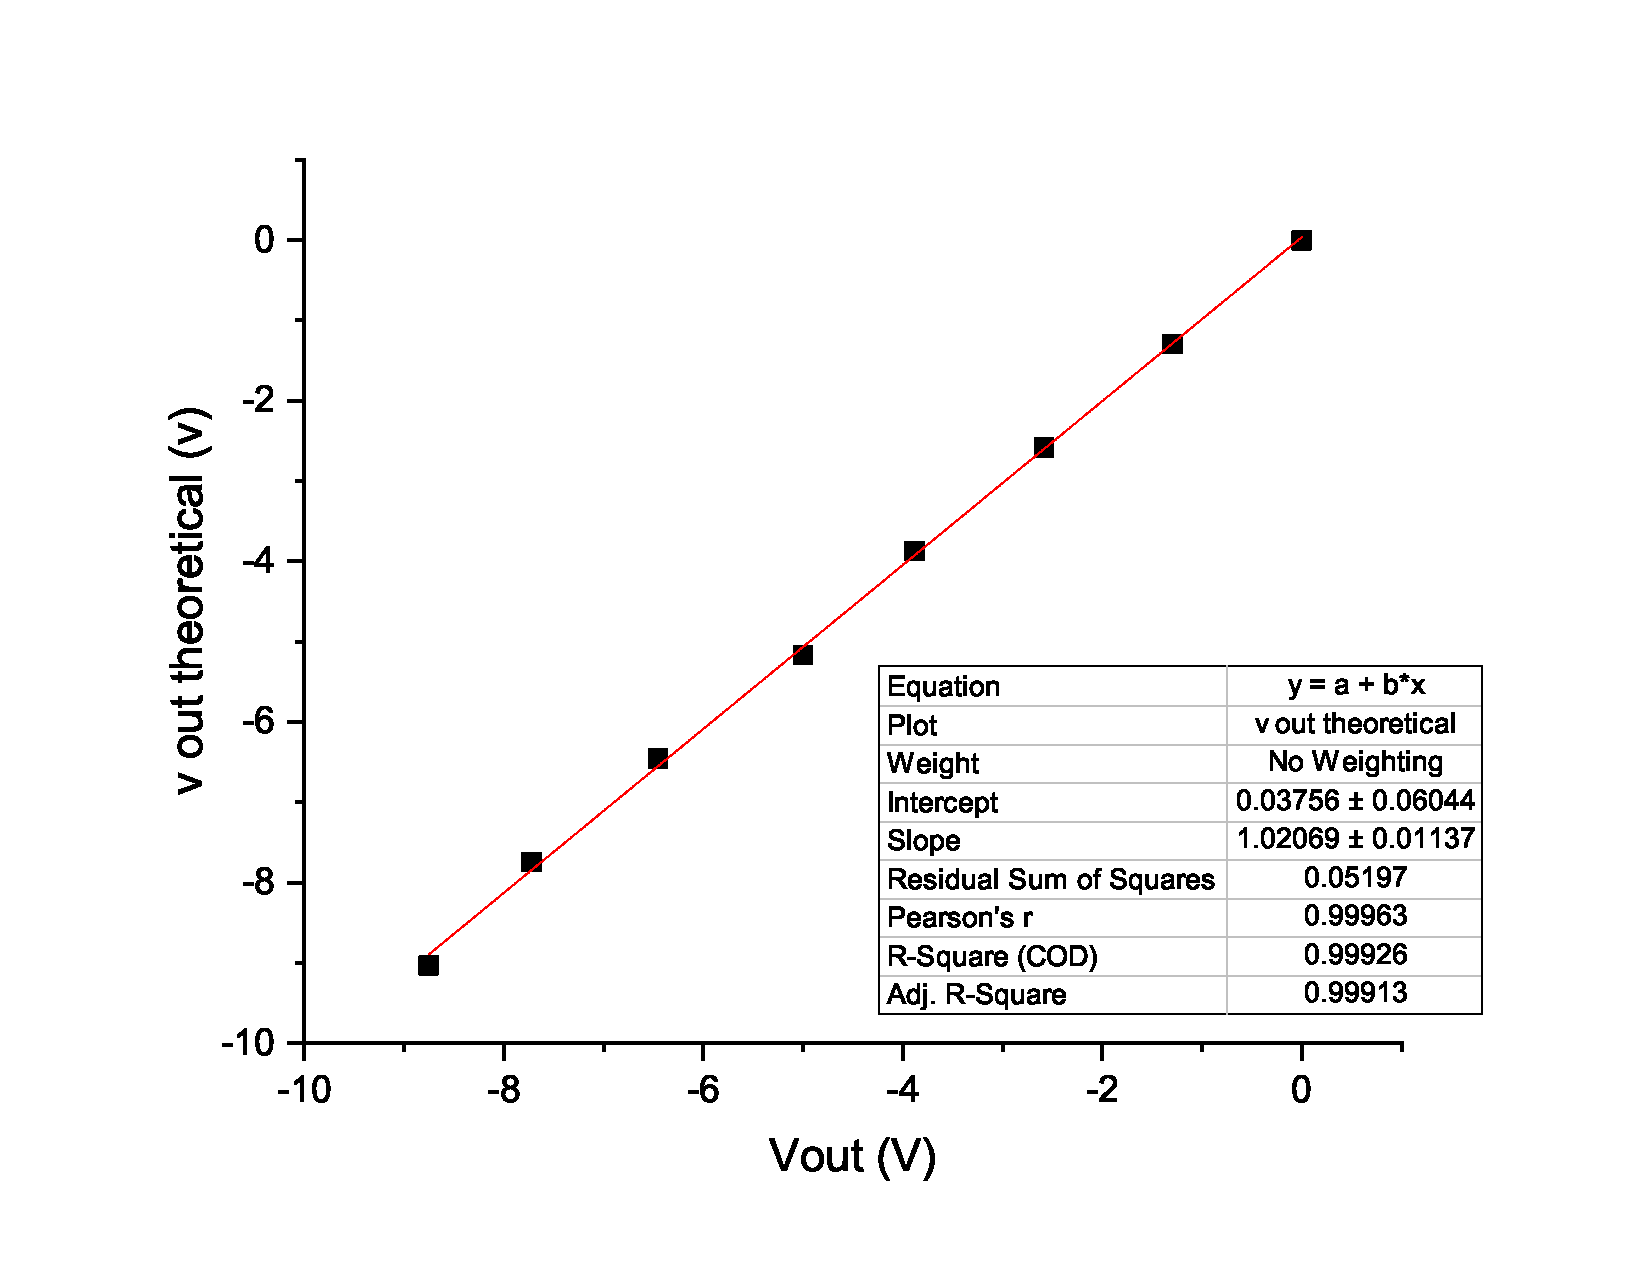
\includegraphics[width=0.8\columnwidth]{images/GR1.eps}
		\caption{$V_{EXP}$ VS $V_{THEORETICAL}$  for DAC }
	\end{figure}
